\documentclass[12pt]{article}
\usepackage{amsmath}
\usepackage{float}
\usepackage{a4wide}
\usepackage{hyperref}
\usepackage{alltt}
\usepackage{tikz}
\usepackage{pgfplots}
\usepackage{calc}
\usepackage[3D]{movie15}
\usepackage{attachfile}
\usepackage{cleveref}

\usetikzlibrary{3d,calc,fadings,decorations.pathreplacing}
\usetikzlibrary{decorations.pathmorphing,decorations.markings,trees,positioning,arrows}
\usetikzlibrary{arrows}
\usetikzlibrary{patterns}

\attachfilesetup{
appearance=true
}

\input{//sol.ita.chalmers.se/groups/bom-kt/VC_Sem/Betongbyggnad_KG/Projekt/1047Klorid_transport/Misc/LaTeX/newcommands_Filip.tex}


\title{Heterogeneous 3D model of concrete}
\begin{document}
\maketitle

\begin{abstract}
Documentation of heterogeneous 3D model of concrete written in MATLAB by \filip. The model implementation solves the heat/diffusion equation both for stationary and transient conditions. All MATLAB code required to use the model is attached to this PDF. Just click the pins to open each \verb|*.m|-file.
\end{abstract}

\tableofcontents

\newpage

\section{MATLAB files}

\subsection{\texttt{SVEGenerator.m} \attachfile[
    icon=PushPin,
    author=SVEGenerator.m,
    description=doubleclick to open in MATLAB
]{\pathtothreede/preprocessor/SVEGenerator.m}
}
\begin{itemize}
\item generates random structured SVE.
\item saves topology data for input to \verb|PreProcessor.m|.
\end{itemize}

\subsection{\texttt{computeDiffusivity.m} \attachfile[
    icon=PushPin,
    author=computeDiffusivity.m,
    description=doubleclick to open in MATLAB
]{\pathtothreede/solvers/computeDiffusivity.m}
}
\begin{itemize}
\item works as a wrapper around LinStatSolver.m and StatPostProcessor.m to compute the 9 components of the homogenized diffusivity tensor.
\item the implementation is parallelized for speed.
\item requires nothing.
\end{itemize}

\subsection{\texttt{PreProcessor.m} \attachfile[
    icon=PushPin,
    author=PreProcessor.m,
    description=doubleclick to open in MATLAB
]{\pathtothreede/preprocessor/PreProcessor.m}
}
\begin{itemize}
\item discretizes SVE to structured grid.
\item creates and saves topology matrices for input to the processor files.
\item requires input data generated by \verb|SVEGenerator.m|.
\end{itemize}


\subsection{\texttt{findITZ.m} \attachfile[
    icon=PushPin,
    author=findITZ.m,
    description=doubleclick to open in MATLAB
]{\pathtothreede/preprocessor/findITZ.m}
}
\begin{itemize}
\item computes $A_\itz, V_\ballast$ and $V_\cement$ in \cref{interfaceVoxel}.
\item called by \verb|PreProcessor.m|.
\end{itemize}

\subsection{\texttt{LinStatSolver.m} \attachfile[
    icon=PushPin,
    author=LinStatSolver.m,
    description=doubleclick to open in MATLAB
]{\pathtothreede/solvers/LinStatSolver.m}
}
\begin{itemize}
\item Solves the linear system of equations, $\ts{K}\ta{a} = \ta{f}$.
\item Dirichlet and convective boundary conditions types are implemented.
\item requires input data generated by \verb|PreProcessor.m|.
\end{itemize}

\subsection{\texttt{LinTransSolver.m} \attachfile[
    icon=PushPin,
    author=LinTransSolver.m,
    description=doubleclick to open in MATLAB
]{\pathtothreede/solvers/LinTransSolver.m}
}
\begin{itemize}
\item Solves the linear system of equations, $\ts{C}\dot{\ta{a}} + \ts{K}\ta{a} = \ta{f}$.
\item convective boundary conditions types are implemented.
\item requires input data generated by \verb|PreProcessor.m|.
\end{itemize}

\subsection{\texttt{StatPostProcessor.m} \attachfile[
    icon=PushPin,
    author=StatPostProcessor.m,
    description=doubleclick to open in MATLAB
]{\pathtothreede/postprocessor/StatPostProcessor.m}
}
\begin{itemize}
\item post processor routine for \verb|LinStatSolver.m|
\item generates \verb|.vtk| file which can be imported to eg Paraview for visualization.
\end{itemize}

\subsection{\texttt{TransPostProcessor.m} \attachfile[
    icon=PushPin,
    author=TransPostProcessor.m,
    description=doubleclick to open in MATLAB
]{\pathtothreede/postprocessor/TransPostProcessor.m}
}
\begin{itemize}
\item post processor routine for \verb|TransStatSolver.m|
\item generates \verb|.vtk| file which can be imported to eg Paraview for visualization.
\end{itemize}


\section{Element node numbering}

\begin{figure}[H]
\centering
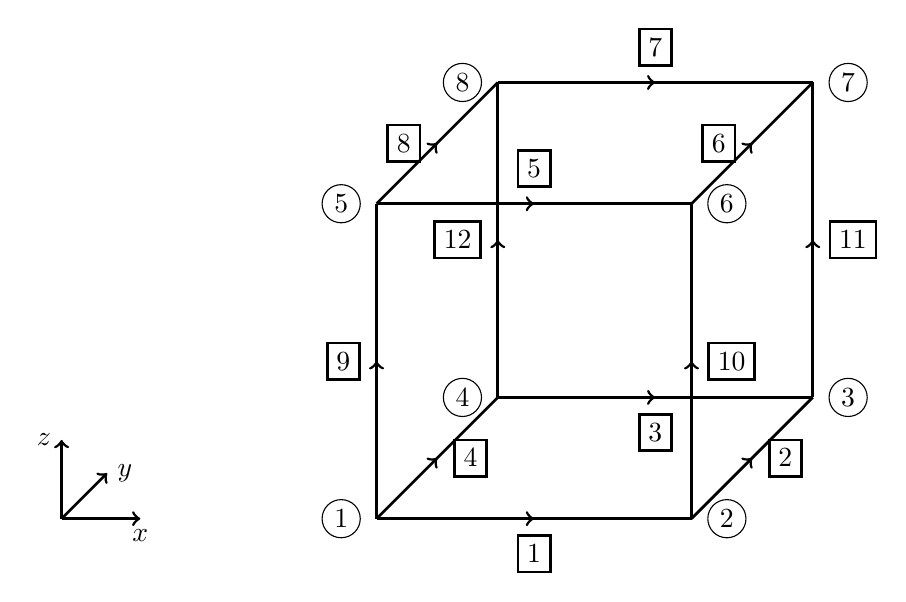
\begin{tikzpicture}[decoration={
    markings,
    mark=at position 0.5 with {\arrow{>}}}]
\pgfmathsetmacro{\cubex}{4}
\pgfmathsetmacro{\cubey}{4}
\pgfmathsetmacro{\cubez}{4}

\coordinate (A) at (0,0,0);
\coordinate (B) at (\cubex,0,0);
\coordinate (C) at (\cubex,0,-\cubez);
\coordinate (D) at (0,0,-\cubez);
\coordinate (E) at (0,\cubey,0);
\coordinate (F) at (\cubex,\cubey,0);
\coordinate (G) at (\cubex,\cubey,-\cubez);
\coordinate (H) at (0,\cubey,-\cubez);


\draw[line width=1pt,->] (-4,0,0) -- (-3,0,0) node[below] {$x$};
\draw[line width=1pt,->] (-4,0,0) -- (-4,1,0) node[left] {$z$};
\draw[line width=1pt,->] (-4,0,0) -- (-4,0,-1.5) node[right] {$y$};


% Segment lines
\draw[line width=1pt,postaction={decorate}] (A) -- (B) node[draw,rectangle,midway,below=2mm] {$1$};
\draw[line width=1pt,postaction={decorate}] (B) -- (C) node[draw,rectangle,midway,right=2mm] {$2$};
\draw[line width=1pt,postaction={decorate}] (D) -- (C) node[draw,rectangle,midway,below=2mm] {$3$};
\draw[line width=1pt,postaction={decorate}] (A) -- (D) node[draw,rectangle,midway,right=2mm] {$4$};

\draw[line width=1pt,postaction={decorate}] (E) -- (F) node[draw,rectangle,midway,above=2mm] {$5$};
\draw[line width=1pt,postaction={decorate}] (F) -- (G) node[draw,rectangle,midway,left=2mm] {$6$};
\draw[line width=1pt,postaction={decorate}] (H) -- (G) node[draw,rectangle,midway,above=2mm] {$7$};
\draw[line width=1pt,postaction={decorate}] (E) -- (H) node[draw,rectangle,midway,left=2mm] {$8$};

\draw[line width=1pt,postaction={decorate}] (A) -- (E) node[draw,rectangle,midway,left=2mm] {$9$};
\draw[line width=1pt,postaction={decorate}] (B) -- (F) node[draw,rectangle,midway,right=2mm] {$10$};
\draw[line width=1pt,postaction={decorate}] (C) -- (G) node[draw,rectangle,midway,right=2mm] {$11$};
\draw[line width=1pt,postaction={decorate}] (D) -- (H) node[draw,rectangle,midway,left=2mm] {$12$};

% Node numbering
\begin{scope}[nodes={inner sep=2pt,draw,circle}]
\node[left=2mm] at (A) {$1$};
\node[right=2mm] at (B) {$2$};
\node[right=2mm] at (C) {$3$};
\node[left=2mm] at (D) {$4$};
\node[left=2mm] at (E) {$5$};
\node[right=2mm] at (F) {$6$};
\node[right=2mm] at (G) {$7$};
\node[left=2mm] at (H) {$8$};
\end{scope}

\end{tikzpicture}
\caption{Node numbers in circles and line segments in rectangles.}
\end{figure}


\section{ITZ implementation}


\begin{figure}[H]
\centering
\scalebox{1.5}{
\begin{tikzpicture}
\pgfmathsetmacro{\cubex}{2}
\pgfmathsetmacro{\cubey}{2}
\pgfmathsetmacro{\cubez}{2}

\coordinate (A) at (0,0,0);
\coordinate (B) at (\cubex,0,0);
\coordinate (C) at (\cubex,0,-\cubez);
\coordinate (D) at (0,0,-\cubez);
\coordinate (E) at (0,\cubey,0);
\coordinate (F) at (\cubex,\cubey,0);
\coordinate (G) at (\cubex,\cubey,-\cubez);
\coordinate (H) at (0,\cubey,-\cubez);


\draw[dashed,line width=1pt] (A) -- (D) -- (C);
\draw[dashed,line width=1pt] (D) -- (H);

\path[fill=gray,opacity=0.3] ($(A)!.30!(E)$) -- ($(B)!.45!(F)$) -- (F) -- (E) -- cycle;
\path[fill=gray,opacity=0.3] ($(B)!.45!(F)$) -- ($(C)!.55!(G)$) -- (G) -- (F) -- cycle;
\path[fill=gray,opacity=0.3] (E) -- (F) -- (G) -- (H) -- cycle;

\draw[line width=1pt] (A) -- (B) -- (F) -- (E) -- cycle;
\draw[line width=1pt] (B) -- (C) -- (G) -- (F);
\draw[line width=1pt] (G) -- (H) -- (E);

% Normal
\draw[|->, >=stealth] ($(A)!.50!(G)$) -- ++(-75:1.0) node[below] {$\ts{n}$};

\path[fill=black] ($(A)!.25!(E)$) -- ($(A)!.30!(E)$) -- ($(B)!.45!(F)$) -- ($(B)!.40!(F)$) -- cycle;
\path[fill=black] ($(B)!.40!(F)$) -- ($(B)!.45!(F)$) -- ($(C)!.55!(G)$) -- ($(C)!.50!(G)$) -- cycle;

\path[fill=black,opacity=0.3] ($(A)!.30!(E)$) -- ($(B)!.45!(F)$) -- ($(C)!.55!(G)$) -- ($(D)!.40!(H)$) -- cycle;
\draw[line width=1pt] ($(A)!.30!(E)$) -- ($(B)!.45!(F)$) -- ($(C)!.55!(G)$) -- ($(D)!.40!(H)$) -- cycle;
\path[pattern=north west lines, pattern color=black] ($(A)!.30!(E)$) -- ($(B)!.45!(F)$) -- ($(C)!.55!(G)$) -- ($(D)!.40!(H)$) -- cycle;


% Annotation
\draw[o-] ($(E)!.50!(G)$) .. controls +(80:0.5) and +(180:0.5) .. ($(B)!1.60!(F)$) node[right] {$V_\ballast$};
\draw[o-] ($(B)!.20!(G)$) .. controls +(0:0.5) and +(180:0.5) .. (3,0.5) node[right] {$V_\cement$};
\draw[o-] ($(A)!.55!(G)$) .. controls +(45:0.5) and +(180:0.5) .. ($(E)!1.50!(F)$) node[right] {$A_\itz$};
\draw[|<->|,>=stealth] (A) ++(-90:0.5) -- ++(0:2) node[fill=white,midway] {$h$};
\draw[|<-,>=stealth] ($(A)!.25!(E)$) ++(180:0.32) -- ++(-90:0.4);
\draw[|<-,>=stealth] ($(A)!.30!(E)$) ++(180:0.32) -- ++(90:0.4) node[left] {$t$};


\end{tikzpicture}
}
\caption{Interface voxel.}
\label{interfaceVoxel}
\end{figure}

\subsection{Line-sphere intersection}

\begin{align}
d = -(\ta{l}\cdot(\ta{o}-\ta{c})) \pm \sqrt{(\ta{l}\cdot(\ta{o}-\ta{c}))^2 - (\ta{o}-\ta{c})^2 +r^2}
\end{align}

\subsection{Voigt assumption}

\subsubsection{Isotropic}
\begin{align}
\bar{D} = \frac{1}{2}(D_\text{a}+D_\text{c}) + \frac{t}{h}D_\text{ITZ}
\end{align}

\subsubsection{Anisotropic}
\begin{align}
\bar{\ts{D}} = \frac{V_\text{a}D_\text{a} + V_\text{c}D_\text{c}}{V_\text{a}+V_\text{c}}\ts{I} + \frac{A_\text{ITZ}D_\text{ITZ}t}{V_\text{a}+V_\text{c}}\left(\ts{I} - \ta{n}\otimes\ta{n}\right)
\end{align}



\end{document} 